\documentclass{report}
\usepackage{geometry}
\usepackage{array}
\usepackage{float}
\usepackage{graphicx}
\usepackage{amsmath}
\usepackage{textcomp}
\usepackage{amssymb}
\usepackage[table]{xcolor}

\begin{document}

\title{Harvard 5 Stages Pipeline CPU Report}
\date{\today}
\maketitle

\section{Contributors information}
\begin{center}
\begin{tabular}{|c|c|c|}
\hline
\textbf{Name} & \textbf{Section} & \textbf{ID} \\
\hline
Youssef Tarek & 2 & 9220990 \\
Marwan Mohamed & 2 & 9220808 \\
Youssef Roshdy & 2 & 9220985 \\
Moamen Hefny & 2 & 9220886 \\
\hline
\end{tabular}
\end{center}

\tableofcontents
\chapter{Introduction}
This is the introduction section of the report. Here you can provide an overview of the topic, background information, and the purpose of the report.

\chapter{Instruction Set Architecture}

\section*{Instruction Types and Classification}
This document defines the instruction set architecture (ISA) for a hypothetical processor. The instructions are categorized into three main types: \textbf{R-Type}, \textbf{I-Type}, and \textbf{J-Type}, with an additional category for miscellaneous instructions referred to as \textbf{Others}. The bit allocation for each instruction type is detailed along with the format used for decoding.

\section*{Instruction Categories}

\subsection*{R-Type (Register-to-Register Instructions)}
R-Type instructions perform operations between registers and store the result in a destination register. They typically involve arithmetic and logical operations.

\[
\begin{array}{|c|c|c|c|c|}
\hline
\text{Opcode} & \text{Function} & \text{Rsrc1} & \text{Rsrc2} & \text{Rdst} \\
\hline
\text{[15-14]} & \text{[13-11]} & \text{[10-8]} & \text{[7-5]} & \text{[4-2]} \\
\hline
\end{array}
\] \\

\textbf{Unused bits:} [1-0]

\textbf{Function field:} 3 bits to specify the operation.

\textbf{Supported Instructions:}
\begin{itemize}
    \item \texttt{NOT Rdst, Rsrc1}
    \item \texttt{INC Rdst, Rsrc1}
    \item \texttt{MOV Rdst, Rsrc1}
    \item \texttt{ADD Rdst, Rsrc1, Rsrc2}
    \item \texttt{SUB Rdst, Rsrc1, Rsrc2}
    \item \texttt{AND Rdst, Rsrc1, Rsrc2}
\end{itemize}

\subsection*{I-Type (Immediate and Memory Instructions)}
I-Type instructions involve immediate values or memory access, typically for arithmetic or data transfer operations.

\[
\begin{array}{|c|c|c|c|c|}
\hline
\text{Opcode} & \text{Function} & \text{Rsrc1} & \text{Rsrc2} & \text{Rdst} \\
\hline
\text{[15-14]} & \text{[13-11]} & \text{[10-8]} & \text{[7-5]} & \text{[4-2]} \\
\hline
\end{array}
\]

\textbf{Unused bits:} [1-0]

\textbf{Second Fetch (Immediate or Offset):}
\[
\begin{array}{|c|}
\hline
\text{Immediate / Offset} \\
\hline
\text{[15-0]} \\
\hline
\end{array}
\]

\textbf{Supported Instructions:}
\begin{enumerate}
    \item \texttt{IADD Rdst, Rsrc1, Imm}
    \item \texttt{LDM Rdst, Imm}
    \item \texttt{LDD Rdst, offset(Rsrc1)}
    \item \texttt{STD Rsrc1, offset(Rsrc2)}
\end{enumerate}

\subsection*{J-Type (Control Flow Instructions)}
J-Type instructions handle program control flow, such as jumps and calls.

\[
\begin{array}{|c|c|c|c|}
\hline
\text{Opcode} & \text{Function} & \text{Rsrc1} & \text{Index} \\
\hline
\text{[15-14]} & \text{[13-11]} & \text{[10-8]} & \text{[7-6]} \\
\hline
\end{array}
\]

\textbf{Unused bits:} [5-0]

\textbf{Supported Instructions:}
\begin{enumerate}
    \item \texttt{JZ Rsrc1}
    \item \texttt{JN Rsrc1}
    \item \texttt{JC Rsrc1}
    \item \texttt{JMP Rsrc1}
    \item \texttt{CALL Rsrc1}
    \item \texttt{RET}
    \item \texttt{RTI}
    \item \texttt{INT index}
\end{enumerate}

\subsection*{Other Instructions}
These instructions do not fit into the R-Type, I-Type, or J-Type categories and typically control processor state or interact with peripherals.

\[
\begin{array}{|c|c|c|c|}
    \hline
    \text{Opcode} & \text{Function} & \text{Rsrc1} & \text{Rdst} \\
    \hline
    \text{[15-14]} & \text{[13-11]} & \text{[10-8]} & \text{[7-5]} \\
    \hline
\end{array}
\]

\textbf{Unused bits:} [4-0]

\textbf{Supported Instructions:}
\begin{enumerate}
    \item \texttt{NOP} – No operation.
    \item \texttt{HLT} – Halt the processor.
    \item \texttt{SETC} – Set the carry flag.
    \item \texttt{OUT Rsrc1} – Output data from \texttt{Rsrc1}.
    \item \texttt{IN Rdst} – Input data into \texttt{Rdst}.
    \item \texttt{PUSH Rsrc1} – Push \texttt{Rsrc1} onto the stack.
    \item \texttt{POP Rdst} – Pop value from the stack into \texttt{Rdst}.
\end{enumerate}

\section*{Bit Allocation Overview}
\begin{itemize}
    \item \textbf{Opcode:} 2 bits \texttt{[15-14]}.
    \item \textbf{Function:} 3 bits \texttt{[13-11]}.
    \item \textbf{Register Fields:}
    \begin{itemize}
        \item \texttt{Rsrc1}: 3 bits \texttt{[10-8]}.
        \item \texttt{Rsrc2}: 3 bits \texttt{[7-5]} (R-Type and I-Type).
        \item \texttt{Rdst}: 3 bits \texttt{[4-2]} (R-Type, I-Type, and Others).
    \end{itemize}
\end{itemize}

\section*{Encoding Summary}
\subsection*{R-Type Encoding}
Utilizes two registers as sources and one destination register. The function field specifies the operation.
\[
\text{[Opcode | Function | Rsrc1 | Rsrc2 | Rdst | Unused(2 bits)]}
\]

\subsection*{I-Type Encoding}
Involves one source register and one destination register, with a second fetch for immediate values or offsets.
\[
\text{[Opcode | Function | Rsrc1 | Rsrc2 | Rdst | Unused(2 bits)]}
\]
\[
\text{[Immediate/Offset (Second Fetch)]}
\]

\subsection*{J-Type Encoding}
Uses a single register as the jump target.
\[
\text{[Opcode | Function | Rsrc1 | Index | Unused(6 bits)]}
\]

\subsection*{Other Instructions Encoding}
Instructions that do not fit into the R-Type, I-Type, or J-Type categories.
\[
\text{[Opcode | Function | Rsrc1 | Rdst | Unused(5 bits)]}
\]


\chapter{Instruction Set Encoding}

\section*{R-Type Instructions}
\begin{table}[H]
    \centering
    \begin{tabular}{|c|c|c|c|c|c|c|}
    \hline
    \textbf{Instruction} & \textbf{Opcode} & \textbf{Function} & \textbf{Rsrc1} & \textbf{Rsrc2} & \textbf{Rdst} & \textbf{Unused} \\ \hline
    NOT Rdst, Rsrc1 & 00 & 000 & xxx & \cellcolor{red!20}000 & xxx & \cellcolor{red!20}00 \\ \hline
    INC Rdst, Rsrc1 & 00 & 001 & xxx & \cellcolor{red!20}000 & xxx & \cellcolor{red!20}00 \\ \hline
    MOV Rdst, Rsrc1 & 00 & 010 & xxx & \cellcolor{red!20}000 & xxx & \cellcolor{red!20}00 \\ \hline
    ADD Rdst, Rsrc1, Rsrc2 & 00 & 011 & xxx & xxx & xxx & \cellcolor{red!20}00 \\ \hline
    SUB Rdst, Rsrc1, Rsrc2 & 00 & 100 & xxx & xxx & xxx & \cellcolor{red!20}00 \\ \hline
    AND Rdst, Rsrc1, Rsrc2 & 00 & 101 & xxx & xxx & xxx & \cellcolor{red!20}00 \\ \hline
    \end{tabular}
    \caption{R-Type Instructions}
    \label{tab:r-type}
\end{table}

\section*{I-Type Instructions}
\begin{table}[H]
    \centering
    \begin{tabular}{|c|c|c|c|c|c|c|}
    \hline
    \textbf{Instruction} & \textbf{Opcode} & \textbf{Function} & \textbf{Rsrc1} & \textbf{Rsrc2} & \textbf{Rdst} & \textbf{Unused} \\ \hline
    IADD Rdst, Rsrc1, Imm & 01 & 000 & xxx & \cellcolor{red!20}000 & xxx & \cellcolor{red!20}00 \\ \hline
    LDM Rdst, Imm & 01 & 001 & 000 & \cellcolor{red!20}000 & xxx & \cellcolor{red!20}00 \\ \hline
    LDD Rdst, offset(Rsrc1) & 01 & 010 & xxx & \cellcolor{red!20}000 & xxx & \cellcolor{red!20}00 \\ \hline
    STD Rsrc1, offset(Rsrc2) & 01 & 011 & xxx & xxx & \cellcolor{red!20}000 & \cellcolor{red!20}00 \\ \hline
    \end{tabular}
    \caption{I-Type Instructions}
    \label{tab:i-type}
\end{table}

\section*{J-Type Instructions}
\begin{table}[H]
    \centering
    \begin{tabular}{|c|c|c|c|c|c|}
    \hline
    \textbf{Instruction} & \textbf{Opcode} & \textbf{Function} & \textbf{Rsrc1} & \textbf{Index} & \textbf{Unused} \\ \hline
    JZ Rsrc1 & 10 & 000 & xxx & \cellcolor{red!20}00 & \cellcolor{red!20}00000000 \\ \hline
    JN Rsrc1 & 10 & 001 & xxx & \cellcolor{red!20}00 & \cellcolor{red!20}00000000 \\ \hline
    JC Rsrc1 & 10 & 010 & xxx & \cellcolor{red!20}00 & \cellcolor{red!20}00000000 \\ \hline
    JMP Rsrc1 & 10 & 011 & xxx & \cellcolor{red!20}00 & \cellcolor{red!20}00000000 \\ \hline
    CALL Rsrc1 & 10 & 100 & xxx & \cellcolor{red!20}00 & \cellcolor{red!20}00000000 \\ \hline
    RET & 10 & 101 & \cellcolor{red!20}000 & \cellcolor{red!20}00 & \cellcolor{red!20}00000000 \\ \hline
    RTI & 10 & 110 & \cellcolor{red!20}000 & \cellcolor{red!20}00 & \cellcolor{red!20}00000000 \\ \hline
    INT index & 10 & 111 & \cellcolor{red!20}000 & xx & \cellcolor{red!20}00000000 \\ \hline
    \end{tabular}
    \caption{J-Type Instructions}
    \label{tab:j-type}
\end{table}


\section*{Other Instructions}
\begin{table}[H]
    \centering
    \begin{tabular}{|c|c|c|c|c|c|}
    \hline
    \textbf{Instruction} & \textbf{Opcode} & \textbf{Function} & \textbf{Rsrc1} & \textbf{Rdst} & \textbf{Unused} \\ \hline
    NOP & 11 & 000 & \cellcolor{red!20}000 & \cellcolor{red!20}000 & \cellcolor{red!20}00000 \\ \hline
    HLT & 11 & 001 & \cellcolor{red!20}000 & \cellcolor{red!20}000 & \cellcolor{red!20}00000 \\ \hline
    SETC & 11 & 010 & \cellcolor{red!20}000 & \cellcolor{red!20}000 & \cellcolor{red!20}00000 \\ \hline
    OUT Rsrc1 & 11 & 011 & xxx & \cellcolor{red!20}000 & \cellcolor{red!20}00000 \\ \hline
    IN Rdst & 11 & 100 & \cellcolor{red!20}000 & xxx & \cellcolor{red!20}00000 \\ \hline
    PUSH Rsrc1 & 11 & 101 & xxx & \cellcolor{red!20}000 & \cellcolor{red!20}00000 \\ \hline
    POP Rdst & 11 & 110 & \cellcolor{red!20}000 & xxx & \cellcolor{red!20}00000 \\ \hline
    \end{tabular}
    \caption{Other Instructions}
    \label{tab:other-instructions}
\end{table}

\section*{Control Unit Signals}
\begin{table}[H]
    \centering
    \begin{tabular}{|c|c|}
    \hline
    \textbf{Instruction} & \textbf{Control Signals} \\ \hline
    \texttt{NOT Rdst, Rsrc1} & \texttt{ALUOp = NOT, RegWrite = 1} \\ \hline
    \texttt{INC Rdst, Rsrc1} & \texttt{ALUOp = INC, RegWrite = 1} \\ \hline
    \texttt{MOV Rdst, Rsrc1} & \texttt{ALUOp = MOV, RegWrite = 1} \\ \hline
    \texttt{ADD Rdst, Rsrc1, Rsrc2} & \texttt{ALUOp = ADD, RegWrite = 1} \\ \hline
    \texttt{SUB Rdst, Rsrc1, Rsrc2} & \texttt{ALUOp = SUB, RegWrite = 1} \\ \hline
    \texttt{AND Rdst, Rsrc1, Rsrc2} & \texttt{ALUOp = AND, RegWrite = 1} \\ \hline
    \texttt{IADD Rdst, Rsrc1, Imm} & \texttt{ALUOp = ADD, ALUSrc2 = 1[Imm], RegWrite = 1, prevOp = 1} \\ \hline
    \texttt{LDM Rdst, Imm} & \texttt{MemRead = 1, ALUSrc2 = 1[Imm]} \\ \texttt{} & \texttt{MemToReg = 1, RegWrite = 1, prevOp = 1} \\ \hline
    \texttt{LDD Rdst, offset(Rsrc1)} & \texttt{MemRead = 1, ALUSrc2 = 1[Imm]} \\ \texttt{} & \texttt{MemToReg = 1, RegWrite = 1, prevOp = 1} \\ \hline
    \texttt{STD Rsrc1, offset(Rsrc2)} & \texttt{MemWrite = 1, ALUSrc2 = 1[Imm], prevOp = 1} \\ \hline
    \texttt{JZ Rsrc1} & \texttt{JZ = 1} \\ \hline
    \texttt{JN Rsrc1} & \texttt{JN = 1} \\ \hline
    \texttt{JC Rsrc1} & \texttt{JC = 1} \\ \hline
    \texttt{JMP Rsrc1} & \texttt{JMP = 1} \\ \hline
    \texttt{CALL Rsrc1} & \texttt{CALL = 1, RegWrite = 1, SP = SP - 1} \\ \hline
    \texttt{RET} & \texttt{JMP = 1, SP = SP + 1} \\ \hline
    \texttt{RTI} & \texttt{JMP = 1, SP = SP + 1} \\ \hline
    \texttt{INT index} & \texttt{INT = 1} \\ \hline
    \texttt{NOP} & \texttt{NOP = 1} \\ \hline
    \texttt{HLT} & \texttt{-} \\ \hline
    \texttt{SETC} & \texttt{CF = 1} \\ \hline
    \texttt{OUT Rsrc1} & \texttt{OUTPORT = 1} \\ \hline
    \texttt{IN Rdst} & \texttt{INPORT = 1, RegWrite = 1} \\ \hline
    \texttt{PUSH Rsrc1} & \texttt{SP = SP - 1} \\ \hline
    \texttt{POP Rdst} & \texttt{RegWrite = 1, SP = SP + 1} \\ \hline
    \end{tabular}
    \caption{Control Unit Signals for Each Instruction}
    \label{tab:cu-signals}
\end{table}

\chapter{Pipeline Stages Design}
The processor pipeline is composed of five distinct stages: \textbf{IF} (Instruction Fetch), \textbf{ID} (Instruction Decode), \textbf{EX} (Execution), \textbf{MEM} (Memory Access), and \textbf{WB} (Write Back). Each stage is responsible for specific tasks in the instruction execution process.

\section*{IF (Instruction Fetch)}
\begin{minipage}{0.6\textwidth}
\begin{itemize}
    \item Fetch the instruction from memory using the Program Counter (PC).
    \item Increment the PC to point to the next instruction.
    \item Store the fetched instruction in the Instruction Register (IR).
    \item Update the PC accordingly in case of a branch or jump instruction.
    \item Stall the PC counter value in case of a halting instruction to stop fetching new instructions.
\end{itemize}
\end{minipage}
\hspace{1cm}
\begin{minipage}{0.35\textwidth}
\begin{center}
    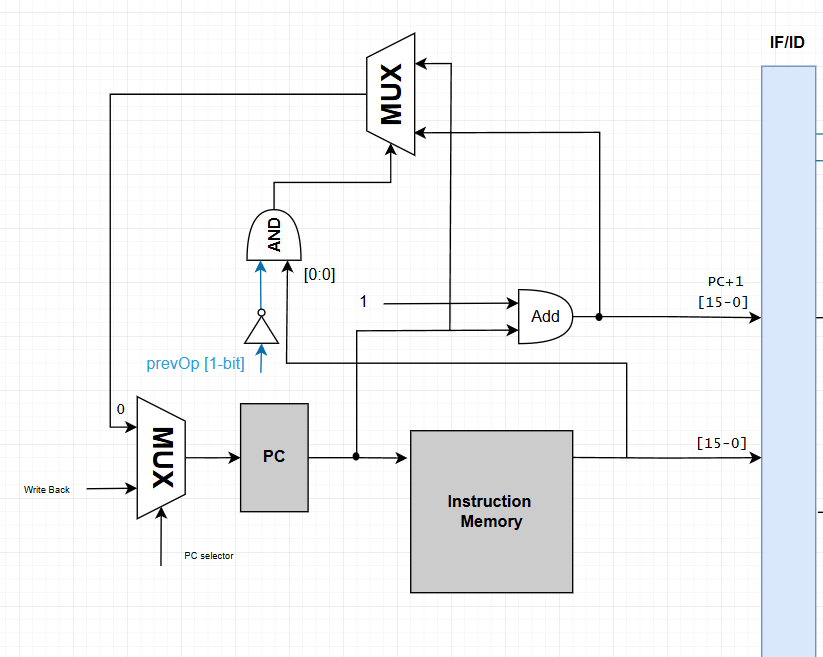
\includegraphics[width=\textwidth]{./assets/IF.png}
\end{center}
\end{minipage}

\section*{ID (Instruction Decode)}
\begin{minipage}{0.6\textwidth}
\begin{itemize}
    \item Decode the instruction opcode and extract the necessary fields.
    \item Read the register file to obtain the values of the source registers.
    \item Determine the type of instruction and generate the required control signals.
    \item Calculate the effective address for memory operations if applicable.
    \item Forward register values and immediate operands to the next stage (EX).
    \item Stall the pipeline if a data hazard is detected and cannot be resolved with forwarding.
\end{itemize}
\end{minipage}
\hspace{1cm}
\begin{minipage}{0.35\textwidth}
\begin{center}
    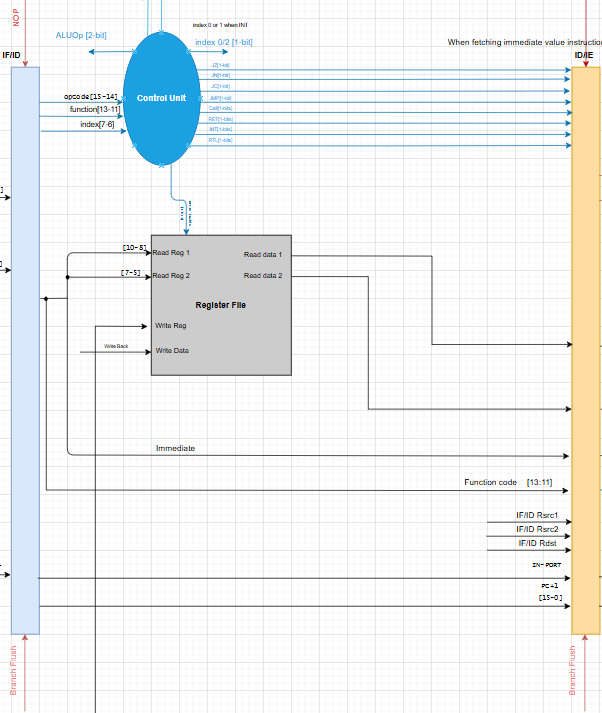
\includegraphics[width=\textwidth]{./assets/ID.png}
\end{center}
\end{minipage}

\section*{EX (Execution)}
\begin{minipage}{0.6\textwidth}
\begin{itemize}
    \item Select ALU inputs through multiplexers based on control signals (\texttt{ALUsrc1} and \texttt{ALUsrc2}).
    \item Perform the ALU operation based on the control signals (\texttt{ALUOp}) and the instruction’s function field (\texttt{Func[3-bit]}).
    \item Generate the condition flags (\texttt{ZF, NF, CF}) based on the ALU result.
    \item Calculate the branch target address if the instruction is a branch or jump.
    \item Evaluate the branch condition using flags and control signals (\texttt{JMP}, \texttt{CALL}, \texttt{JC}, \texttt{JZ}, \texttt{JN}).
    \item Forward the ALU result to the Memory Access (MEM) stage.
    \item Stall the pipeline if a data hazard is detected and cannot be resolved with data forwarding.
    \item Flush the pipeline if a branch instruction is mispredicted.
    \item Generate control signals to update the Program Counter (PC) if a branch is taken.
\end{itemize}
\end{minipage}
\hspace{1cm}
\begin{minipage}{0.35\textwidth}
\begin{center}
    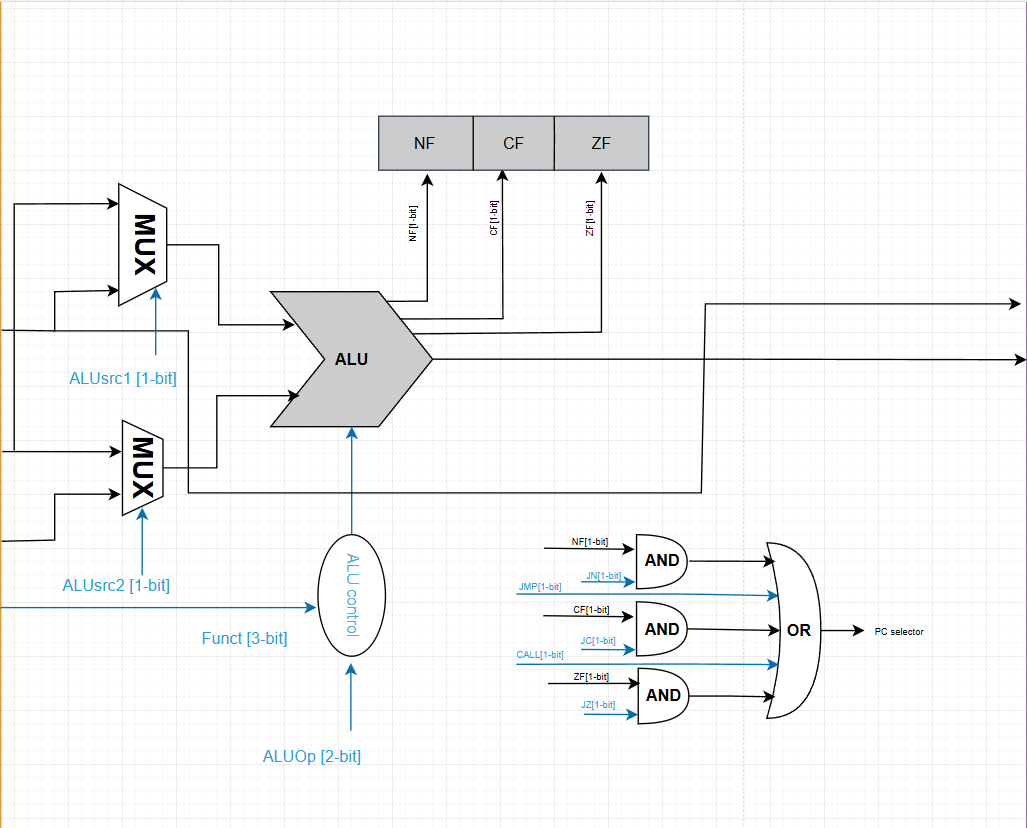
\includegraphics[width=\textwidth]{./assets/EX.png}
\end{center}
\end{minipage}

\section*{MEM (Memory Access)}
\begin{minipage}{0.6\textwidth}
\begin{itemize}
    \item Access memory to read or write data based on the instruction type.
    \item Forward the memory read data to the Write Back (WB) stage.
    \item Stall the pipeline if a data hazard is detected and cannot be resolved with data forwarding.
    \item Handle stack operations (PUSH, POP) through the stack control unit.
    \item Generate signals to enable memory read/write operations.
    \item Forward the ALU result to the WB stage if the instruction does not involve memory access.
\end{itemize}
\end{minipage}
\hspace{1cm}
\begin{minipage}{0.35\textwidth}
\begin{center}
    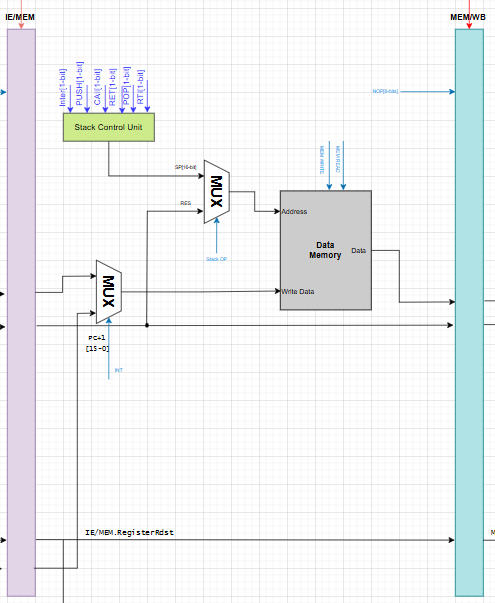
\includegraphics[width=\textwidth]{./assets/MEM.png}
\end{center}
\end{minipage}

\section*{WB (Write Back)}
\begin{minipage}{0.6\textwidth}
\begin{itemize}
    \item Update the register file with the new value if the instruction is a register operation.
    \item Update the Program Counter (PC) with the branch target address if a branch is taken.
    \item Stall the pipeline if a data hazard is detected and cannot be resolved with data forwarding.
    \item Update the PC with the target address if the instruction is a jump or call.
    \item Update the PC with the return address if the instruction is a return.
    \item Halt the processor if the instruction is a halt.
\end{itemize}
\end{minipage}
\hspace{1cm}
\begin{minipage}{0.35\textwidth}
\begin{center}
    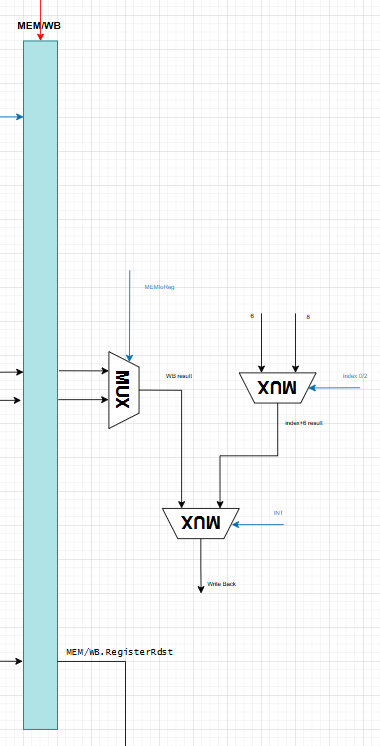
\includegraphics[width=\textwidth]{./assets/WB.png}
\end{center}
\end{minipage}

\chapter{Hazard Handling}

\section*{Handling Structural Hazards}
Structural hazards are managed by ensuring that the pipeline has enough resources to handle multiple instructions simultaneously. This can be achieved by duplicating resources or by scheduling instructions to avoid conflicts.

\subsection*{Resource Duplication}
Duplicating critical resources, such as ALUs or memory ports, allows multiple instructions to use these resources concurrently, reducing the likelihood of structural hazards.

\subsection*{Instruction Scheduling}
To further mitigate structural hazards, we have chosen to schedule the read and write operations in different parts of the cycle. This approach ensures that:
\begin{itemize}
    \item \textbf{Write Operations:} Are performed in the first half of the clock cycle.
    \item \textbf{Read Operations:} Are performed in the second half of the clock cycle.
\end{itemize}
By separating read and write operations within the same cycle, we minimize resource conflicts and improve the overall efficiency of the pipeline.

\section*{Handling Data Hazards}
Data hazards are managed using data forwarding and pipeline stalling:
\begin{itemize}
    \item \textbf{Data Forwarding:} The result of an instruction is forwarded to subsequent instructions that need it before it is written back to the register file.
    \item \textbf{Pipeline Stalling:} The pipeline is stalled until the required data is available. This is done by inserting no-operation (NOP) instructions.
\end{itemize}

\subsection*{Example of Data Forwarding}
Consider the following sequence of instructions:
\begin{verbatim}
    ADD R1, R2, R3              IF     ID     EX --|  MEM     WB
    SUB R4, R1, R5              -      IF     ID   |->EX      MEM     WB
\end{verbatim}
The result of the ADD instruction is forwarded to the SUB instruction to avoid stalling the pipeline.

\subsection*{Example of Pipeline Stalling}
Consider the following sequence of instructions:
\begin{verbatim}
    LDD R1, 0(R2)               IF     ID     EX      MEM --|  WB
    ADD R3, R1, R4              -      IF     ID------ID    |->EX      MEM     WB 
\end{verbatim}
The pipeline is stalled until the LDD instruction completes and the data is available for the ADD instruction.

\section*{Handling Control Hazards}
Control hazards are handled using branch prediction techniques. We employ a static branch prediction technique known as "Backward Taken, Forward Not Taken" (BTFNT). This technique predicts that a branch will be taken if it jumps backward (typically for loops) and not taken if it jumps forward.

\subsection*{Backward Taken, Forward Not Taken (BTFNT)}
The BTFNT technique helps in reducing the number of pipeline flushes by making educated guesses about the branch direction based on its target address.

\subsection*{Example of BTFNT}
Consider the following sequence of instructions:
\begin{verbatim}
    LOOP:   SUB R1, R1, #1          IF     ID     EX     MEM     WB
            JNZ LOOP                -      IF     ID     EX      MEM     WB
            IN Rsrc2   --flush      -      -      IF
\end{verbatim}
In this example, the branch instruction `JNZ LOOP` jumps backward to the label `LOOP`. Using BTFNT, the pipeline predicts that the branch will be taken.

\begin{verbatim}
    ADD R2, R3, R4                 IF     ID     EX     MEM     WB
    JMP END                        -      IF     ID     EX      MEM     WB
    SUB R5, R6, R7     --flush     -      -      IF
    END:   HLT                     -      -      -      IF      ID      EX      MEM     WB
\end{verbatim}
In this example, the branch instruction `JMP END` jumps forward to the label `END`. Using BTFNT, the pipeline predicts that the branch will not be taken.

\subsection*{Pipeline Flushing}
If the prediction is incorrect, the pipeline is flushed, and the correct instructions are fetched. This involves invalidating the instructions in the pipeline stages and fetching the correct instructions from memory.

\subsection*{Advantages of BTFNT}
\begin{itemize}
    \item Effective for typical loop structures and forward jumps.
    \item Reduces the number of pipeline flushes compared to always predicting taken or not taken.
\end{itemize}

\section*{Pipeline Hazard Detection Unit}
A hazard detection unit is implemented to identify hazards and take appropriate actions. It monitors the pipeline stages and generates control signals to handle hazards.

\begin{center}
\begin{minipage}{0.75\textwidth}
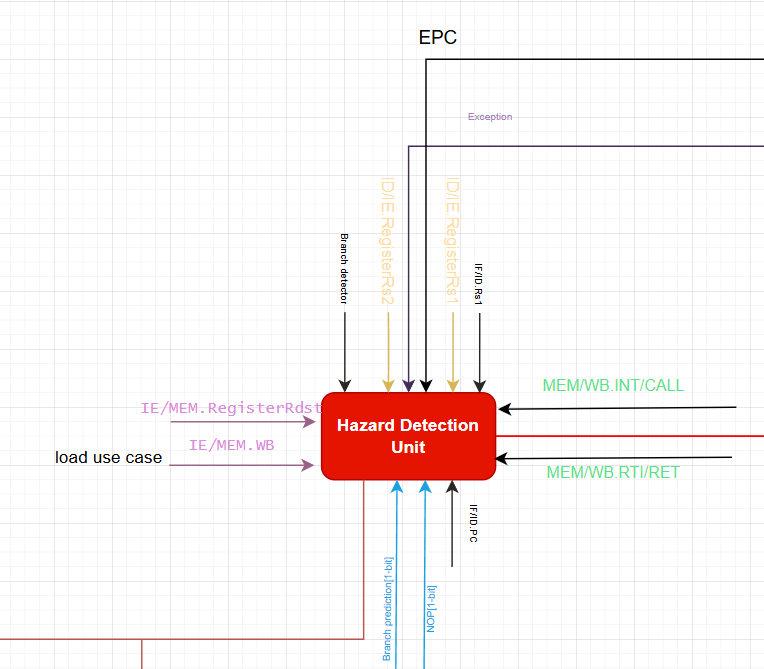
\includegraphics[width=\textwidth]{./assets/HDU.png}
\end{minipage}
\end{center}

\begin{itemize}
    \item \textbf{Structural Hazard Detection:} Ensures that the pipeline has enough resources to handle multiple instructions simultaneously by duplicating resources or scheduling instructions to avoid conflicts.
    \item \textbf{Data Hazard Detection:} Manages data hazards using data forwarding to pass results directly to dependent instructions or pipeline stalling by inserting no-operation (NOP) instructions until the required data is available.
    \item \textbf{Control Hazard Detection:} Uses branch prediction techniques, specifically "Backward Taken, Forward Not Taken" (BTFNT), to predict branch directions and manage pipeline flushing if the prediction is incorrect.
\end{itemize}

\chapter{Exception Handling}

\section*{Exception Types}
Exceptions are unexpected events that occur during program execution, requiring special handling to ensure the correct operation of the processor. The following exception types are supported by the processor: \\

\begin{itemize}
    \item \textbf{Stack Underflow:} Occurs when the stack pointer exceeds its limits.
    \item \textbf{Invalid Memory Access:} Indicates an attempt to access an invalid memory location.
\end{itemize}

\begin{center}
    \begin{minipage}{0.75\textwidth}
    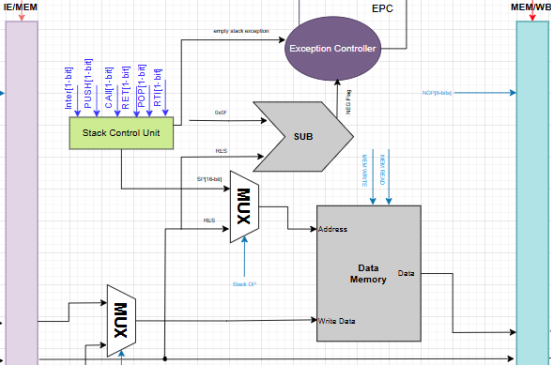
\includegraphics[width=\textwidth]{./assets/EC.png}
    \end{minipage}
    \end{center}
\end{document}
